\documentclass{article}
\usepackage[utf8]{inputenc}
\usepackage[T1]{fontenc}
\usepackage{amsmath}
\usepackage{tikz}
\usetikzlibrary{positioning}
\usetikzlibrary{arrows.meta,arrows}

\begin{document}

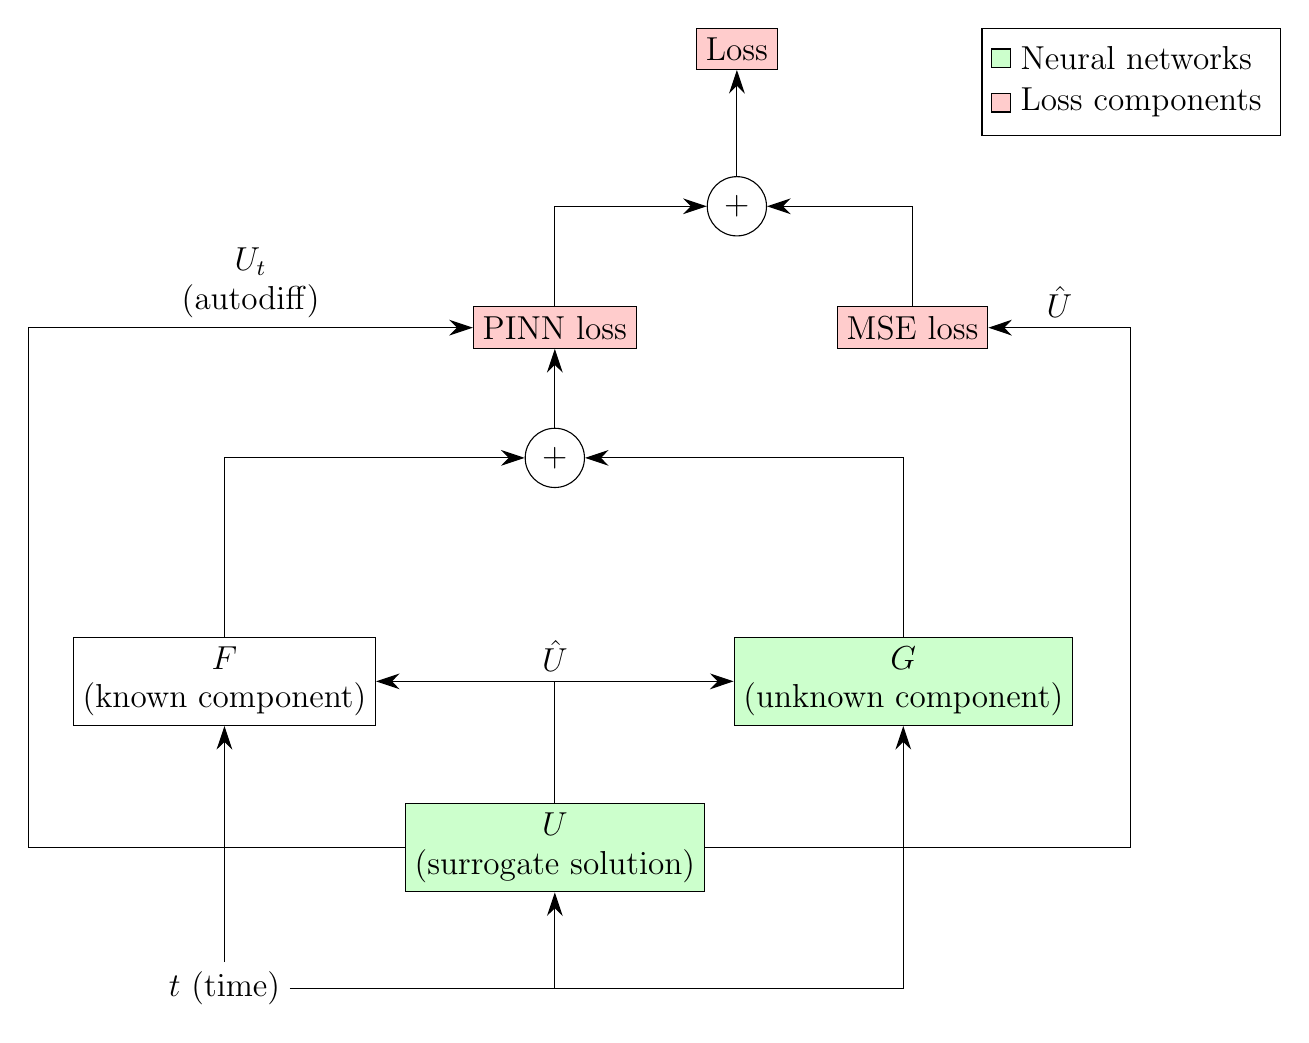
\begin{tikzpicture}[greennode/.style={shape=rectangle, fill=green, draw=black, fill opacity=0.2,text opacity=1.0,align=center},
rednode/.style={shape=rectangle, fill=red, draw=black, fill opacity=0.2,text opacity=1.0,align=center}
,font=\sffamily]
\tikzstyle{every node}=[font=\large]
  \node[circle,draw] (add_1) at (0,0) {$+$};
  \node[rednode]  (loss) at (0,2)  {Loss};

  \node[rednode] (pinn_loss) [below left=1cm and 1cm of add_1]  {PINN loss};% 2cm below, 1cm to the left (optional)
  \node[circle,draw] (add_2) [below=1cm of pinn_loss] {$+$};
  \node[rednode] (mse_loss) [below right=1cm and 1cm of add_1] {MSE loss};
  \node[rectangle,draw,align=center]  (G) [below left=2cm and 2cm of add_2]  {$F$\\(known component)};
  \node[greennode]  (F) [below right=2cm and 2cm of add_2]  {$G$ \\(unknown component)};
  \node[rectangle,draw,align=center,fill=green, fill opacity=0.2,text opacity=1.0]  (U) [below=4cm of add_2]  {$U$ \\(surrogate solution)};
  \node  (t) [below=3cm of G]  {$t$ (time)};
  \draw [-{Stealth[length=3mm, width=2mm]}] (mse_loss) |- (add_1);
  \draw [-{Stealth[length=3mm, width=2mm]}] (pinn_loss) |- (add_1);
  \draw [-{Stealth[length=3mm, width=2mm]}] (G) |- (add_2);
  \draw [-{Stealth[length=3mm, width=2mm]}] (F) |- (add_2);
  \draw [-{Stealth[length=3mm, width=2mm]}] (add_1) -- (loss);
  \draw [-{Stealth[length=3mm, width=2mm]}] (add_2) -- (pinn_loss);
  \draw [-{Stealth[length=3mm, width=2mm]}] (U.north) |- (F.west) node[midway,above] {$\hat{U}$} ;
  \draw [-{Stealth[length=3mm, width=2mm]}] (U.north) |- (G.east) ;
  \draw [-{Stealth[length=3mm, width=2mm]}] (t) -- (G);
  \draw [-{Stealth[length=3mm, width=2mm]}] (t.east) -| (U);
  \draw [-{Stealth[length=3mm, width=2mm]}] (t.east) -| (F);
  \draw [-{Stealth[length=3mm, width=2mm]}] (U.east) -| (5,-5) |- (mse_loss.east) node[pos=0.75,above,align=center] {$\hat{U}$};
  \draw [-{Stealth[length=3mm, width=2mm]}] (U.west) -| (-9,-5)  |- (pinn_loss.west) node[pos=0.75,above,align=center] {$U_t$ \\ (autodiff)};
  \matrix [draw, below] at (current bounding box.north east) {
    \node [greennode,label=right:Neural networks] {}; \\
    \node [rednode,label=right:Loss components] {}; \\
  };
  \end{tikzpicture}

\end{document}